\documentclass[a4paper,11pt]{article}
\setlength{\textwidth}{15.93cm} \setlength{\textheight}{24.61cm}
\oddsidemargin=-0.0cm \topmargin=-1.33cm
\usepackage{charter,eulervm}
\renewcommand{\baselinestretch}{1.1}
\usepackage{amsthm,amsmath,amssymb,upgreek,marvosym}
\usepackage{makeidx}  % allows for indexgeneration
\usepackage{paralist}
\usepackage{subcaption}
\usepackage{caption}
\usepackage{tabularx}
\usepackage[usenames,dvipsnames]{color}
\usepackage[pdftex,breaklinks,colorlinks,
    citecolor={blue}, linkcolor={blue},urlcolor=Maroon]{hyperref}
\usepackage{tkz-graph}
\usetikzlibrary{arrows,shapes,decorations.pathmorphing,positioning, fit, calc}

\graphicspath{{./images/}}%helpful if your graphic files are in another directory
%
\theoremstyle{plain} %remark,  plain
\newtheorem{theorem}{Theorem}[section]
\newtheorem{lemma}[theorem]{Lemma}
\newtheorem{corollary}[theorem]{Corollary}
\newtheorem{proposition}[theorem]{Proposition}
\newtheorem{definition}{Definition}
\def\boxit#1{\vbox{\hrule\hbox{\vrule\kern4pt
  \vbox{\kern1pt#1\kern1pt}
\kern2pt\vrule}\hrule}}

\newcommand{\keywords}[1]{\bigskip \par\noindent
{\small{\em Keywords\/}: #1}}
\newcommand{\opt}[2]{\ensuremath{{\mathtt{#1}(#2)}}}
\newcommand{\comment}[1]{\`$\setminus\!\!\setminus${\em #1}}

\title{\vspace{-2cm}COMP4134 - Biometrics and Security \\ Assignment 2 Report}
\author{
	Xiating Ouyang 14111773D \\
	Yuanjing Shi 13104584D \\
	Fengming Liu 15104126D \\
	Wenqi Jia 15102855D \\
	Yufan Zhuang 14110419D \\
	}
\date{}

\begin{document}
\maketitle	

\section{Introduction}
Retina is an ideal biometric for security purposes for the complexity of vessels in the retina and the impossibility to alter retina through surgeries. In this report, we investigate the state-of-the-art retina recognition algorithm on open databases of retina images and evaluate its performance.

\section{Retina recognition glossories}

\subsection{Performance}
The retina recognition algorithms have been intensively investigated. However, their performance evaluation results are largely limited due to the insufficient retina images available. For example, an algorithm utilizing the correlation and covariance matrix can achieve 100\% recongition rate on 20 images, when the testing data is the same as the training data \cite{kakarwal2010analysis}. Other attempts include using the Artificial Neural Networks (ANN) and Fuzzy Inference, which achieves an identification rate of 93\% and 96\%, respectively \cite{borah2015retina}.


\subsection{Applications}
Retina recognition can be used as a biometric feature to ensure the security of entities and institution. The acquisition of a retina sample requires the user to peep into an eyepiece for a relatively long time for the system to acurately capture an image of the retina, which adversely affect the usability of this system. However, due to its high accuracy in recognition, it has been utilized by government agencies including the Federal Bureau of Investigation (FBI), the Central Intelligence Agency (CIA) and the National Aeronautics and Space Administration (NASA). Apart from its security-related applications, it is also applied in medical institutions to detect hereditary diseases.

\subsection{Database availability}

The STARE (STructured Analysys of the Retina) Project started in 1975, aiming at developing a facilitating tool for ophthalmologists to automatically diagnose diseases. There are around 400 raw images available at http://cecas.clemson.edu/$\sim$ahoover/stare/, with the limitation that no clear label of identity is provided. See sample from Figure \ref{fig1}.
\begin{figure}
	\begin{subfigure}{0.4\textheight}
		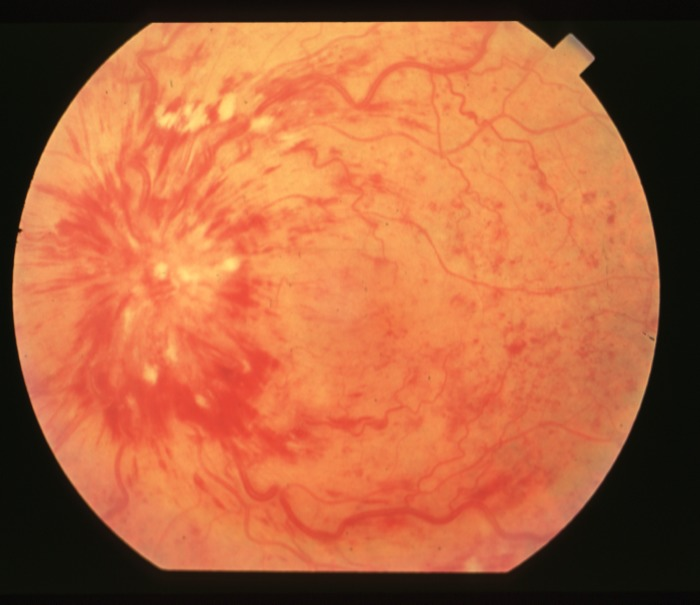
\includegraphics[width=0.4\linewidth]{im0019}
		\caption{Sample from the STARE database}
		\label{fig1}
	\end{subfigure}
    \begin{subfigure}{0.4\textheight}
		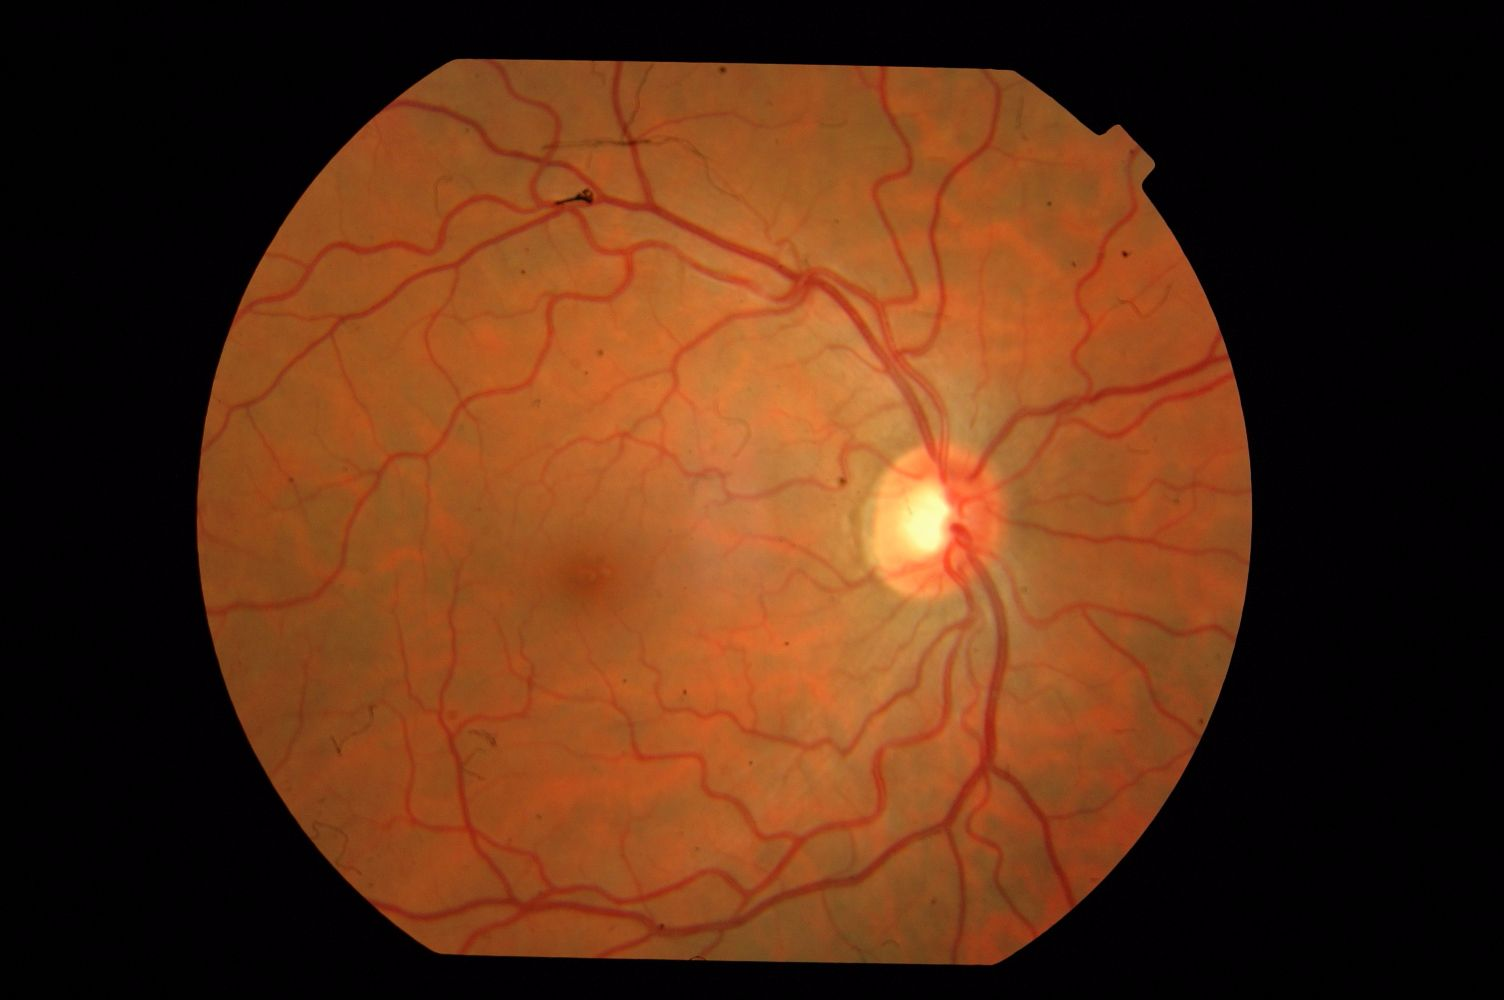
\includegraphics[width=0.4\linewidth]{IM000003_17}
		\caption{Sample from the VARPA database}
		\label{fig2}
	\end{subfigure}

\end{figure}

The VARPA database is an open database storing 233 images from 139 individuals, and is accessible at http://www.varpa.es/research/biometrics.html\#databases. Full access has to be granted by the owner, Dr. Marcos Ortega Hortas. We were granted access to the database on November 6, 2017. See sample from Figure \ref{fig2}.

The DRIVE database has been established to enable comparative studies on segmentation of blood vessels in retinal images. The research community is invited to test their algorithms on this database and share the results with other researchers through this web site.


\subsection{Acquisition devices}
Retina recognition is essentially to study the retinal vascular pattern hidden within our eyes, which is shown not to have the tendency to change while aging \cite{fatima2013feature}. 


It is a common practice that retina imaging would conducted by an ophthalmologist, a medical doctor that specializes in the function, diseases, and structure of the human eye, during a process of a clinical examination. An optical camera is used to see through the pupil of the eye to the rear inner surface of the eyeball. A picture is taken showing the optic nerve, fovea, surrounding vessels, and the retinal layer.

To be more specific, take DRIVE the retinal image database for vessel extraction as an example, the photographs for the DRIVE database were obtained from a diabetic retinopathy screening program in The Netherlands. The screening population consisted of 400 diabetic subjects between 25-90 years of age. The images were acquired using a Canon CR5 non-mydriatic 3CCD camera with a 45 degree field of view (FOV). Each image was captured using 8 bits per color plane at 768 by 584 pixels. The FOV of each image is circular with a diameter of approximately 540 pixels. For this database, the images have been cropped around the FOV. For each image, a mask image is provided that delineates the FOV.

\subsection{Remedies insufficient subject images}
Since most of the public retina databases are for medical usage only, normally only one image is captured for each subject, thereby leaving a difficulty to compute genuine and imposter distribution. Dias et al. \cite{dias2014retinal} suggests that the retina image captured are prone to brightness and unpredicted noise variations. Therefore, we would simulate such changes to manually produce images that are of the same person but with different qualities. 



\section{Performance evaluation}

\subsection{Execution}

\subsection{Graphical summaries}

\subsection{Further improvements}


\section{Concluding remarks}
In this project, we have thoroughly investigated the retina recognition methods. Its applications and acquisition methods are also revisited. We have also tested the state-of-the-art algorithm using the publically available databases and produced preliminary performance summary for the algorithm. Future refinement to the algorithm would include using some [random bullshiting techniques] to further improve the accuracy of retina recognition. Meanwhile, it is also an opportunity to create more advanced devices than the currently available ones to provide convenience to acquire the retina sample.


\bibliographystyle{unsrt}
\bibliography{report}
\end{document}